While it would be interesting to progressively transect the ligament in order to simulate chronic deterioration, in the interest of time only two stages will be used: native laxity and \SI{10}{mm}, as measured in a simulated Lachman test.

\paragraph{Technique}
The native state of the ACL and its deterioration are quantified through a simulated Lachman test. 
The Lachman test outlines 3 grades based on the displacement of the tibia relative to the femur: 1 (0–-5 mm), 2 (6–-10 mm) or 3 (11–-15 mm).
A grade of 2 or above is indicative of AP laxity.

For small increases of AP laxity, a mixture of partial transections and pie-crusting \cite{clarke_clinical_2005} will be utilised, targeting the anteromedial bundle (areas G, H in figure \ref{fig:am-pl-bundle}) \cite{kawaguchi_role_2015}.
% Additional guidance on pie-crust or transect can be found in the works of Kagawuchi \cite{kawaguchi_role_2015} and Yamakawa \cite{yamakawa_strain_2017}.
\begin{figure}[]\centering
    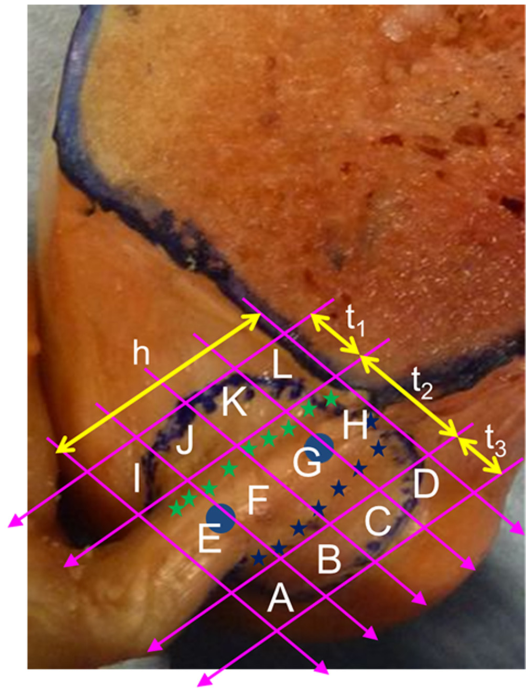
\includegraphics[width=0.3\textwidth]{figures/am-pl-bundles}
    \caption{Sections G,H roughly correspond to AM bundles \cite{kawaguchi_role_2015}}
\label{fig:am-pl-bundle}
\end{figure}
